Before delving into universality for random matrices we explore the scalar random variable version: the Central Limit Theorem (CLT). You would have already seen the \emph{Normal distribution} $\ensuremath{\scrN}$ (with mean zero and variance one), which has a Probability Density Function (PDF) which is a Gaussian:
\[
{\E^{-x^2/2} \over \sqrt{2\ensuremath{\pi}}}.
\]
The CLT is the fundamental result that when we add many independent samples of a random number it behaves like a Normal distribution. More precisely, if $X_1,\ensuremath{\ldots},X_n$ are all iid and (for simplicity) have zero mean and variance:
\meeq{
\ensuremath{\bbE} X_k = 0, \qquad
\ensuremath{\bbE} X_k^2 = 1,
}
then we claim that the rescaled sum
\[
S_n := {X_1 + \ensuremath{\cdots} + X_n \over \sqrt{n}}.
\]
looks like $\ensuremath{\scrN}$ as $n \ensuremath{\rightarrow} \ensuremath{\infty}$.

We will show this using the Method of Moments: we want to show the moments $\ensuremath{\bbE} S_n^k$ tend to the moments of $\ensuremath{\scrN}$. When moments do not grow too fast, convergence in moments tells us convergence in probability densities (the precise details of this are beyond the scope of these notes), so it suffices to show convergence of moments to establish the CLT.  This argument serves as a blueprint for a similar Method of Moments that can be used to prove universality for random matrices.

\section{Experimental observation of the Central Limit Theorem}
Consider sampling iid discrete random variables $X_1,\ensuremath{\ldots},X_n$ each taking values $\ensuremath{\pm}1$ with equal probability, so that their expectation is zero and variance is one:
\meeq{
\ensuremath{\bbE} X_k = (-1) {1 \over 2} + 1 {1 \over 2} = 0, \qquad
\ensuremath{\bbE} X_k^2 = (-1)^2 {1 \over 2} + 1^2 {1 \over 2} = 1.
}
By summing and rescaling these variables we can get a new random variable $S_n$:
\[
S_n := {X_1 + \ensuremath{\cdots} + X_n \over \sqrt{n}}.
\]
For large $n$ we can compare a histogram of samples of $S_n$ to a Gaussian:


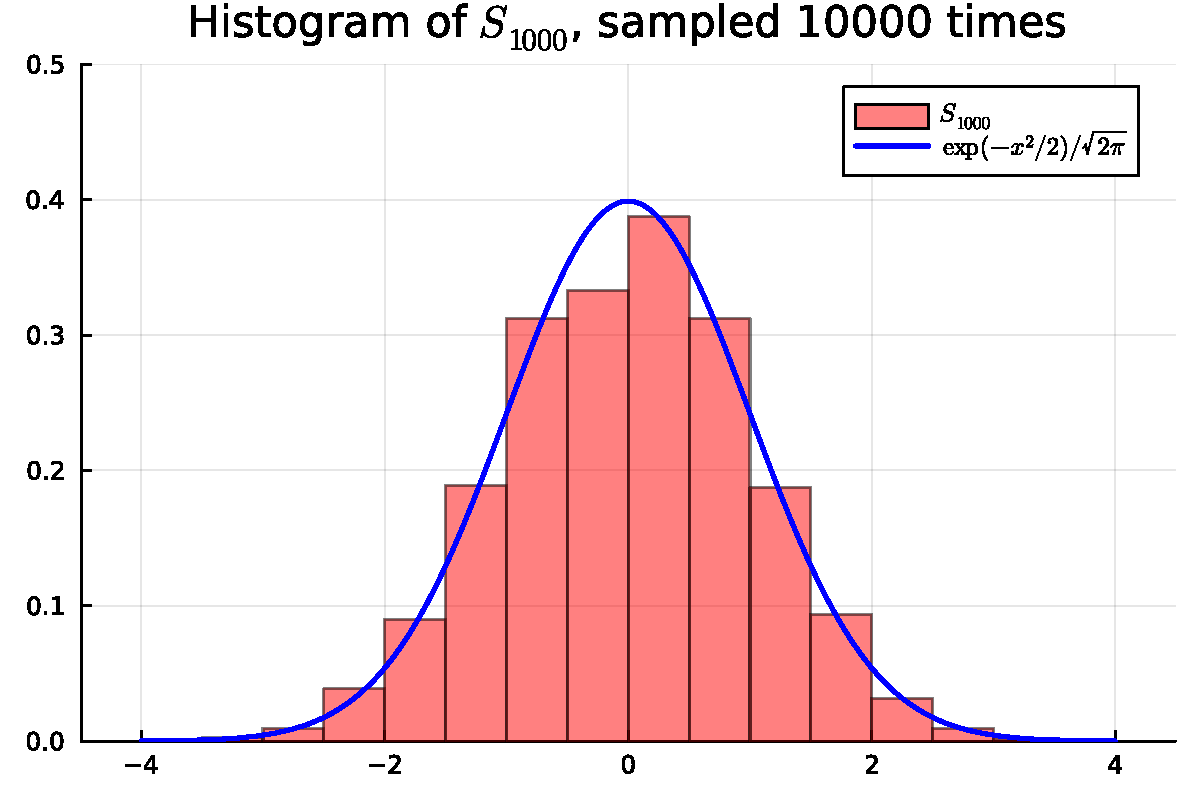
\includegraphics[width=0.6\linewidth,height=0.45\linewidth]{figures/I.CLT_1_1.pdf}

They look very close! In fact, by making $n$ and the number of samples large enough we can make the histogram look arbitrarily close to a Gaussian. This phenomena is independent of the distribution of $X_k$ provided the moments are finite: we always get a normal distribution (shifted and scaled to match the mean and variance).

We are going to show why this phenomena is true using the Method of Moments: we want to show the moment $\ensuremath{\bbE}S_n^k$ tend to the moments of a Normal distribution. We can deduce the moments experimentally by averaging over many samples and letting $n$ increase:


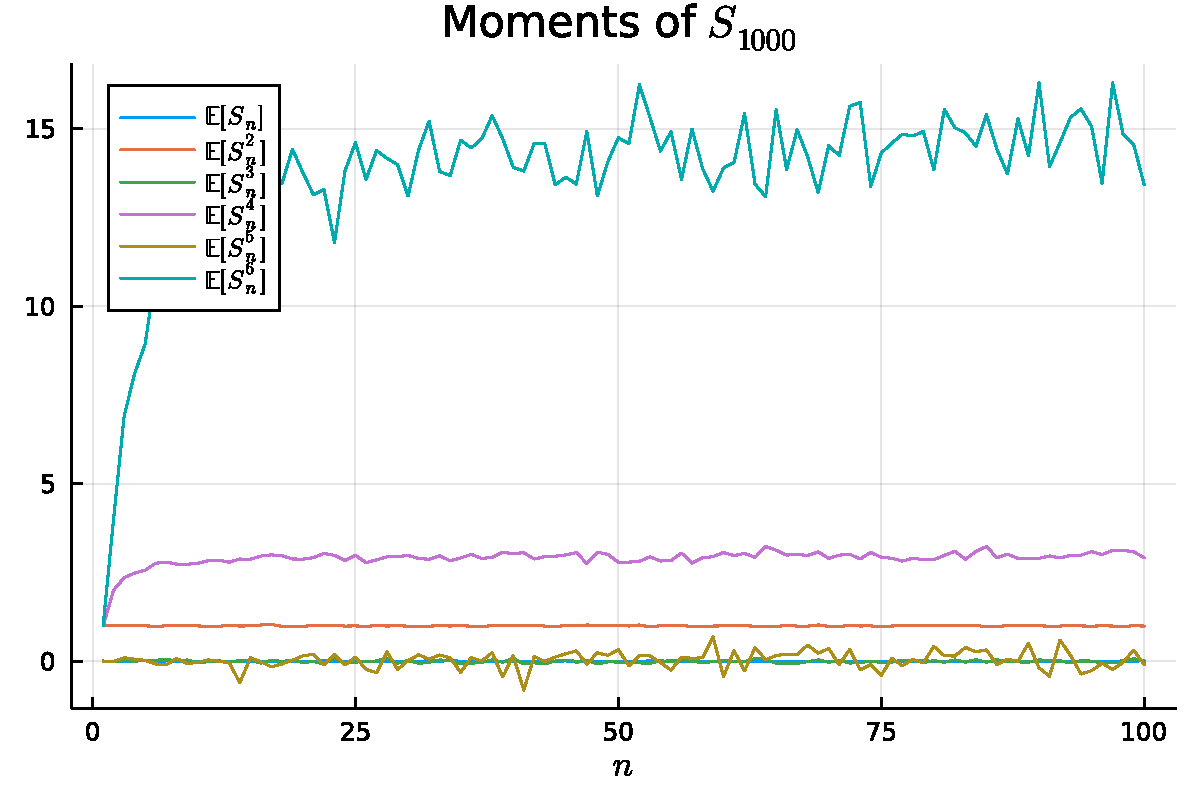
\includegraphics[width=0.6\linewidth,height=0.45\linewidth]{figures/I.CLT_2_1.pdf}

A sensible conjecture then is that $\ensuremath{\bbE}S_n^k$ is zero when $k$ is odd whilst
\[
\ensuremath{\bbE}S_n^2 \ensuremath{\rightarrow} 1,\quad \ensuremath{\bbE}S_n^4 \ensuremath{\rightarrow} 3, \quad \ensuremath{\bbE}S_n^6 \ensuremath{\rightarrow} 15.
\]
Thus we are left with the tasks of: (1) deducing an exact formula for these moments, and (2) proving that the Gaussian has the same moments.

\section{Moments of the normal distribution}
We will use the Method of Moments, so our first step is to establish an explicit formula for the moments of a Normal distribution, i.e., we want to compute
\[
\ensuremath{\mu}_k^N := \ensuremath{\int}_{-\ensuremath{\infty}}^\ensuremath{\infty} x^k {\E^{-x^2/2}  \over \sqrt{2\ensuremath{\pi}}} \dx.
\]
We will relate these integrals to the following combinatorial object:

\begin{definition}[double factorial]
\[
(2m-1)!! := {(2m)! \over 2^m m!} = 1 \ensuremath{\cdot} 3 \ensuremath{\cdot} 5 \ensuremath{\cdots} (2m-1).
\]
\end{definition}

Note this satisfies a simple recurrence:
\[
(2m-1)!! = (2m-1) \ensuremath{\cdot} (2m-3)!! \quad \hbox{for} \quad m > 1.
\]
We can check the first few double factorials:
\[
1!! = 1,\quad 3!! = 3,\quad 5!! = 15
\]
which exactly match our predicted values for the first few even moments $\ensuremath{\bbE}S_n^2,\ensuremath{\bbE}S_n^4,\ensuremath{\bbE}S_n^6$.  We claim this holds true for all even moments: $\ensuremath{\bbE}S_n^{2m} = (2m-1)!!$.

To prove this result we will combine a combinatorial argument (to reduce $\ensuremath{\bbE}S_n^{2m}$ to $(2m-1)!!$) with an integration-by-parts argument (to reduce $\ensuremath{\mu}_{2m}^N$ to $(2m-1)!!$). For the combinatorial argument we note that the double factorial  counts the number of ways to partition $\{1,\ensuremath{\ldots},2m\}$ into $m$ different pairs, that is to write
\[
\{1,\ensuremath{\ldots},2m\} = \{x_1,y_1\} \ensuremath{\cup} \ensuremath{\cdots} \ensuremath{\cup} \{x_m,y_m\}
\]
where $x_1,\ensuremath{\ldots},x_m,y_1,\ensuremath{\ldots},y_m$ is a permutation of $1,\ensuremath{\ldots},2m$ and $x_k < y_k$ for all $k$. For example, if $m = 2$ then we have the following pairings of $1,2,3,4$:
\[
\{1,2\}, \{3,4\} \qquad \{1,3\}, \{2,4\} \qquad \{1,4\}, \{2,3\}
\]
and  $3!! = 3$. And if $m = 3$ then we have $5!! = 15$ total pairings:
\begin{align*}
\{1,2\}, \{3,4\}, \{5,6\} &\qquad \{1,2\}, \{3,5\}, \{4,6\} \qquad \{1,2\}, \{3,6\}, \{4,5\} \\
\{1,3\}, \{2,4\}, \{5,6\} &\qquad \{1,3\}, \{2,5\}, \{4,6\} \qquad \{1,3\}, \{2,6\}, \{4,5\} \\
\{1,4\}, \{2,3\}, \{5,6\} &\qquad \{1,4\}, \{2,5\}, \{3,6\} \qquad \{1,4\}, \{2,6\}, \{3,5\} \\
\{1,5\}, \{2,3\}, \{4,6\} &\qquad \{1,5\}, \{2,4\}, \{3,6\} \qquad \{1,5\}, \{2,6\}, \{3,4\} \\
\{1,6\}, \{2,3\}, \{4,5\} &\qquad \{1,6\}, \{2,4\}, \{3,5\} \qquad \{1,6\}, \{2,5\}, \{3,4\}.
\end{align*}
This relationship holds for all $m$:

\begin{lemma}[pair partitions] The number of partitions of $2m$ into pairs equals $(2m-1)!!$.

\end{lemma}
\textbf{Proof} The relationship between the double factorial and the number of pair partitions can be deduced by a very simple inductive argument. When $m = 1$ we have exactly $1!! = 1$ pairings. If we assume the number of pairings of $2, 4, \ensuremath{\ldots}, 2m$ are given by $3!!,5!!,\ensuremath{\ldots},(2m-1)!!$ then we deduce the number of pairings of $2(m+1)$ as follows. We can pair the first number ($1$) with a choice of the $2m+1$ other numbers ($2,3,\ensuremath{\ldots},$ or $2m+2$). But then by the induction hypothesis the remaining $2m$ numbers have exactly $(2m-1)!!$ pairings. Thus we have
\[
\underbrace{(2m+1)}_{\hbox{Choices for $1$}} \times \underbrace{(2m-1)!!}_{\hbox{Choices for pairing remaining $2m$ elements}} = (2m+1)!!
\]
where the last equality follows from the recurrence for double factorials.

\ensuremath{\QED}

We now show the moments of a Gaussian are also given in terms of the double factorial:

\begin{lemma}[Gaussian moments]
\[
\ensuremath{\mu}_k^N := \ensuremath{\int}_{-\ensuremath{\infty}}^\ensuremath{\infty} x^k {\E^{-x^2/2}  \over \sqrt{2\ensuremath{\pi}}} \dx = \begin{cases}
0 & \hbox{\textrm{if  $k$ is odd}} \\
{(k-1)!!} & \hbox{\textrm{if $k$ is even}}
\end{cases}
\]
\end{lemma}
\textbf{Proof} The case of $k$ odd follows from symmetry. For even $k$ we  use a proof by induction. The base case of $k = 0$ follows using the classic trick of computing the integral of a Gaussian by turning it into a 2D integral, using polar coordinates ($r^2 = x^2 + y^2$) and the change of variables $t = r^2/2$:
\meeq{
\pr(\ensuremath{\int}_{-\ensuremath{\infty}}^\ensuremath{\infty} \E^{-x^2/2} \dx)^2 = \pr(\ensuremath{\int}_{-\ensuremath{\infty}}^\ensuremath{\infty} \E^{-x^2/2} \dx)\pr(\ensuremath{\int}_{-\ensuremath{\infty}}^\ensuremath{\infty} \E^{-y^2/2} \dy) =
\ensuremath{\int}_{-\ensuremath{\infty}}^\ensuremath{\infty} \ensuremath{\int}_{-\ensuremath{\infty}}^\ensuremath{\infty} \E^{-(x^2+y^2)/2} \dx \dy \ccr
= \ensuremath{\int}_0^\ensuremath{\infty} \ensuremath{\int}_0^{2\ensuremath{\pi}}  r \E^{-r^2/2} \dr \D\ensuremath{\theta}  = 2\ensuremath{\pi} \ensuremath{\int}_0^\ensuremath{\infty}  \E^{-t} \dt =2\ensuremath{\pi},
}
hence
\[
\ensuremath{\mu}_0^N = {\ensuremath{\int}_{-\ensuremath{\infty}}^\ensuremath{\infty} \E^{-x^2/2} \dx \over \sqrt{2\ensuremath{\pi}}} = 1.
\]
For even $k> 0$ assume it is true for all smaller $k$. Then we can integrate-by-parts to deduce:
\meeq{
\sqrt{2\ensuremath{\pi}} \ensuremath{\mu}_k^N = \ensuremath{\int}_{-\ensuremath{\infty}}^\ensuremath{\infty} x^k \E^{-x^2/2} \dx = \ensuremath{\int}_{-\ensuremath{\infty}}^\ensuremath{\infty} x^{k-1} \underbrace{x \E^{-x^2/2}}_{=-{\D \over \dx}  \E^{-x^2/2}} \dx \ccr
= [-x^{k-1} \E^{-x^2/2}]_{-\ensuremath{\infty}}^\ensuremath{\infty} + (k-1) \ensuremath{\int}_{-\ensuremath{\infty}}^\ensuremath{\infty} x^{k-2} \E^{-x^2/2} \dx =  \sqrt{2\ensuremath{\pi}} (k-1) \ensuremath{\mu}_{k-2}^N.
}
I.e., $\ensuremath{\mu}_k^N = (k-1) \ensuremath{\mu}_{k-2}^N$, but this is exactly the formula that we showed $(k-1)!!$ satisfies above (if we write $k = 2m$).

\ensuremath{\QED}

\section{Proof of CLT using Method of Moments}
We now want to show that the moments $\ensuremath{\bbE}S_n^k$ for
\[
S_n := {X_1 + \ensuremath{\cdots} + X_n \over \sqrt{n}}.
\]
are also given by the double factorial as $n \ensuremath{\rightarrow} \ensuremath{\infty}$ and hence match the moments of a Normal Distribution.  We show this by relating the moments to the number of pair partitions:

\begin{theorem}[CLT] Let $X_1, X_2, \ensuremath{\ldots}, X_n$ be iid variables with $\ensuremath{\bbE}X_j = 0$, $\ensuremath{\bbE}X_j^2 = 1$, and all other moments are finite. Then for all $k$ we have
\[
\ensuremath{\bbE}S_n^k \underset{n \ensuremath{\rightarrow} \ensuremath{\infty}}{\ensuremath{\longrightarrow}} \ensuremath{\mu}_k^N.
\]
\end{theorem}
\textbf{Proof} We are going to present a slightly unusual argument that mimics the upcoming proof of random matrix universality as much as possible. The $X_j$  are iid and we can write their moments as
\[
\ensuremath{\mu}_k = \ensuremath{\bbE}X_j^k
\]
where $\ensuremath{\mu}_0 = 1$ and by assumption $\ensuremath{\mu}_1 = 0$ and $\ensuremath{\mu}_2 = 1$.

We first note we can naively expand
\[
(X_1 + \ensuremath{\cdots} + X_n)^k = \ensuremath{\sum}_{i_1,\ensuremath{\ldots},i_k=1}^n X_{i_1} \ensuremath{\cdots} X_{i_k},
\]
i.e., a sum with $n^k$ terms. Since we know $X_i$ commute, one angle of proof is to simplify this using the multinomial expansion to combine the terms where the differen $i_\ensuremath{\ell}$ match, but instead we are going to break up the sum according to whether the components are the same or different, which can be identified with partitions of $\{1,\ensuremath{\ldots},n\}$.

Let's walk through some simple cases. For $k= 1$ the result is trivial:
\meeq{
\ensuremath{\bbE}S_n = n^{-1/2} \ensuremath{\sum}_{i=1}^n \ensuremath{\bbE}X_i = 0.
}
For $k = 2$ we consider
\[
\ensuremath{\bbE}S_n^2 = n^{-1} \ensuremath{\sum}_{i_1,i_2=1}^n \ensuremath{\bbE}[X_{i_1}X_{i_2}]
\]
by breaking up the sum over two different cases: either $i_1 = i_2$ or $i_1 \ensuremath{\neq} i_2$.  We can associate these with partitions of $2$ numbers as either $\{1,2\}$ (when they match) or $\{1\}, \{2 \}$ (when they differ). Here is a table of which partitions correspond to which terms, and how many of each type of term we have, where now we assume $i_1 \ensuremath{\neq} i_2$:
\[
\begin{array}{c | c | c}
\hbox{Partition} & \hbox{Term} & \hbox{Count} \\
\hline
  \{1\}, \{2\} & \ensuremath{\bbE}[X_{i_1} X_{i_2}] = \ensuremath{\bbE}X_{i_1} \ensuremath{\bbE}X_{i_2}  = \ensuremath{\mu}_1^2  = 0  & n(n-1) = n^2 + O(n)\\
    \{1,2\} & \ensuremath{\bbE} X_{i_1}^2 = \ensuremath{\mu}_2 = 1 &  n
\end{array}
\]
Note since $n^2 = n + n(n-1)$ we have accounted for all terms. But the only terms that are non-zero are those associated with $\{1,2\}$. Thus we find the second moment reduces to
\[
\ensuremath{\bbE} S_n^2 = n^{-1} \ensuremath{\sum}_{i_1=1}^n  \ensuremath{\bbE} X_{i_1}^2 = 1.
\]
For $n = 3$ we consider
\[
\ensuremath{\bbE}S_n^3 = n^{-3/2} \ensuremath{\sum}_{i_1,i_2,u_3=1}^n \ensuremath{\bbE}[X_{i_1}X_{i_2}X_{i_3}]
\]
by breaking up the cases according to the different partitions of 3 elements based on which terms match, where  now we assume $i_1 \ensuremath{\neq} i_2 \ensuremath{\neq} i_3$:
\[
\begin{array}{c | c | c}
\hbox{Partition} & \hbox{Term} & \hbox{Count} \\
\hline
  \{1\}, \{2\} , \{3\}  & \ensuremath{\bbE}[X_{i_1} X_{i_2} X_{i_3}] =\ensuremath{\mu}_1^3  = 0  &  n(n-1)(n-2) = n^3 + O(n^2) \\
  \{1,2\}, \{3\}  & \ensuremath{\bbE}[X_{i_1}^2 X_{i_3}] =\ensuremath{\mu}_2 \ensuremath{\mu}_1  = 0  & n(n-1) \\
  \{1,3\}, \{2\}  & \ensuremath{\bbE}[X_{i_1}^2 X_{i_2}] =\ensuremath{\mu}_2 \ensuremath{\mu}_1  = 0  & n(n-1) \\
  \{1\}, \{2,3\}  & \ensuremath{\bbE}[X_{i_1} X_{i_2}^2] =\ensuremath{\mu}_1 \ensuremath{\mu}_2  = 0  & n(n-1) \\
  \{1,2,3\}  & \ensuremath{\bbE} X_{i_1}^3 = \ensuremath{\mu}_3   &  n 
\end{array}
\]
We have accounted for all $n^3 = n(n-1)(n-2) + 3n(n-1) + n$ terms and in this case all terms vanish. We do one last explicit example: for $n = 4$ where   we assume $i_1 \ensuremath{\neq} i_2 \ensuremath{\neq} i_3 \ensuremath{\neq} i_4$ we have the following cases:
\[
\begin{array}{c | c | c}
\hbox{Partition} & \hbox{Term} & \hbox{Count} \\
\hline
\{1\}, \{2\}, \{3\}, \{4\} & \ensuremath{\bbE}[X_{i_1} X_{i_2} X_{i_3} X_{i_4}] = \ensuremath{\mu}_1^4 = 0 & n (n-1)(n-2)(n-3) = n^4 + O(n^2) \\
\{1,2\}, \{3\}, \{4\} & \ensuremath{\bbE}[X_{i_1}^2 X_{i_3} X_{i_4}] = \ensuremath{\mu}_2 \ensuremath{\mu}_1^2 = 0 & n(n-1)(n-2)= n^3 + O(n^2) \\
\{1,3\}, \{2\}, \{4\} & \ensuremath{\bbE}[X_{i_1}^2 X_{i_2} X_{i_4}] = \ensuremath{\mu}_2 \ensuremath{\mu}_1^2 = 0 & n(n-1)(n-2) = n^3 + O(n^2)\\
\{1,4\}, \{2\}, \{3\} & \ensuremath{\bbE}[X_{i_1}^2 X_{i_2} X_{i_3}] = \ensuremath{\mu}_2 \ensuremath{\mu}_1^2 = 0 & n(n-1)(n-2) = n^3 + O(n^2)\\
\{1\}, \{2,3\}, \{4\} & \ensuremath{\bbE}[X_{i_1} X_{i_2}^2 X_{i_4}] = \ensuremath{\mu}_1 \ensuremath{\mu}_2 \ensuremath{\mu}_1 = 0 & n(n-1)(n-2) = n^3 + O(n^2)\\
\{1\}, \{2,4\}, \{3\} & \ensuremath{\bbE}[X_{i_1} X_{i_2}^2 X_{i_3}] = \ensuremath{\mu}_1 \ensuremath{\mu}_2 \ensuremath{\mu}_1 = 0 & n(n-1)(n-2) = n^3 + O(n^2)\\
\{1\}, \{2\}, \{3,4\} & \ensuremath{\bbE}[X_{i_1} X_{i_2} X_{i_3}^2] = \ensuremath{\mu}_1^2 \ensuremath{\mu}_2  = 0 & n(n-1)(n-2) = n^3 + O(n^2)\\
\{1,2\}, \{3,4\} &  \ensuremath{\bbE}[X_{i_1}^2 X_{i_3}^2] =\ensuremath{\mu}_2^2 = 1 & n(n-1)=n^2 + O(n) \\
\{1,3\}, \{2,4\} &  \ensuremath{\bbE}[X_{i_1}^2 X_{i_2}^2] =\ensuremath{\mu}_2^2 = 1 & n(n-1)=n^2 + O(n) \\
\{1,4\}, \{2,3\} & \ensuremath{\bbE}[X_{i_1}^2 X_{i_2}^2] =\ensuremath{\mu}_2^2 = 1 & n(n-1)=n^2 + O(n) \\
\{1,2,3\}, \{4\} & \ensuremath{\bbE}[X_{i_1}^3 X_{i_4}] =\ensuremath{\mu}_3 \ensuremath{\mu}_1 = 0 & n(n-1) = n^2 + O(n) \\
\{1,2,4\}, \{3\} & \ensuremath{\bbE}[X_{i_1}^3 X_{i_3}] =\ensuremath{\mu}_3 \ensuremath{\mu}_1 = 0 & n(n-1) = n^2 + O(n) \\
\{1\}, \{2,3,4\} & \ensuremath{\bbE}[X_{i_1} X_{i_2}^3] = \ensuremath{\mu}_1 \ensuremath{\mu}_3 = 0 & n(n-1) = n^2 + O(n) \\
\{1,2,3,4\} & \ensuremath{\bbE}X_{i_1}^4 = \ensuremath{\mu}_4 & n
\end{array}
\]
The only non-zero terms are those of pair partitions (there are $n^2 + O(n)$ of those) and a partition with 4 elements (there are only $n$ of those). Hence we deduce:
\meeq{
\ensuremath{\bbE} S_n^4 = n^{-2} \ensuremath{\sum}_{\hbox{pair partitions}}\qquad \underbrace{n(n-1)}_{\hbox{terms per partition}}\\
&\qquad  + n^{-2} \ensuremath{\sum}_{\hbox{parititions with 4 elements}}\qquad \underbrace{n}_{\hbox{terms per partition}}  \qquad  \ensuremath{\mu}_4 \\
&=
n^{-2} \underbrace{3}_{\hbox{number of pair partitions}} (n^2 + O(n)) + n^{-1} \ensuremath{\mu}_4\\
& \underset{n \ensuremath{\rightarrow} \ensuremath{\infty}}{\ensuremath{\longrightarrow}} 3!!
}
At this point the argument is clear for general $k$. There are $n^k + O(n^{k-1})$ terms where each element differ, corresponding to the partition $\{1\},\ensuremath{\ldots},\{k\}$, but because of independence these all contribute zero because indepedence guarantees:
\[
\ensuremath{\bbE}[X_{i_1} \ensuremath{\cdots} X_{i_k}] = \ensuremath{\mu}_1^k = 0
\]
Each partition with a single pair has associated with it $n^{k-1} + O(n^{k-2})$ terms, but these also vanishes by the same argument since there are terms that appear onde. For even $k$ this continues until we reach exactly $k/2$ pairs, the partition that has no singletons, in which case the moments are
\[
\ensuremath{\bbE}[X_{i_1}^2 \ensuremath{\cdots} X_{i_{k/2}}^2] = \ensuremath{\bbE}X_{i_1}^2 \ensuremath{\cdots} \ensuremath{\bbE}X_{i_{k/2}}^2 = \ensuremath{\mu}_2^{k/2} = 1,
\]
and each possible pairing has $n (n-1) \ensuremath{\cdots} (n-k/2) = n^{k/2} + O(n^{k/2-1})$ terms. Thus the total is
\meeq{
\ensuremath{\bbE} S_n^k = n^{-k/2} \ensuremath{\sum}_{\hbox{pair partitions of $k$}}  \underbrace{[n^{k/2} + O(n^{k/2-1})]}_{\hbox{number of terms per partition}} + O(n^{-1}) \ccr
= (k-1)!! + O(n^{-1}) \\
&\underset{n \ensuremath{\rightarrow} \ensuremath{\infty}}{\ensuremath{\longrightarrow}} (k-1)!!
}
When $k$ is odd, the non-vanishing partition with the most number of terms correspond to a single 3 elements and $(k-3)/2$ pairs. As there are only $n (n-1) \ensuremath{\cdots} (n-(k-3)/2) = n^{(k-1)/2} + O(n^{(k-3)/2})$ of these, the scaling $n^{-k/2}$ dominates and we have
\[
\ensuremath{\bbE} S_n^k = n^{-1/2} + O(n^{-3/2}) \underset{n \ensuremath{\rightarrow} \ensuremath{\infty}}{\ensuremath{\longrightarrow}} 0.
\]
\ensuremath{\QED}

\textbf{Remark} Note the assumption of finite moments is essential. A classic counter example is if $X_k$ have a heavy-tail distribution like the Cauchy distribution:
\[
{1 \over \ensuremath{\pi}} {1 \over x^2 + 1}.
\]
Not even the first moment exists, that is, this distribution has no mean! (Symmetry may make one think that the mean should be zero, but if we average samples it never converges.) If we take iid samples $X_k$ of the Cauchy distribution we know that
\[
{X_1 + \ensuremath{\cdots} + X_n \over n}
\]
is the same Cauchy distribution. (Note the division by $n$, not $\sqrt{n}$, which differs from the CLT above.)

\section{Poster projects}
While I expect most projects to be on random matrices, there are some interesting angles for projects that focus more on the CLT. Here are a few examples:

\begin{itemize}
\item[1. ] Give a detailed explanation of the Method of Moments and a comparison to an alternative analysis-based proof using the moment generating function $\ensuremath{\bbE}\E^{t X}$.


\item[2. ] Explore multiplicative version of the CLT involving rescaled products of positive iid random numbers. What distribution arises as the number of products becomes infinite?


\item[3. ] Exploration (either experimental or mathematical) of the CLT for heavytailed distributions like the Cauchy distribution where the Method of Moments breaks down.

\end{itemize}

